\documentclass[a4paper,11pt]{article}

\usepackage[utf8]{inputenc}
\usepackage[T1]{fontenc}
\usepackage{geometry}
\geometry{margin=2.2cm}
\usepackage{xcolor}
\usepackage{graphicx}
\usepackage{tikz}
\usetikzlibrary{calc}
\usepackage{everypage}
\usepackage{amsmath}
\usepackage{amssymb}
\usepackage{booktabs}
\usepackage{caption}
\usepackage{float}
\usepackage[colorlinks=true,linkcolor=blue,urlcolor=blue]{hyperref}

\setlength{\parskip}{0.6em}
\setlength{\parindent}{0pt}

\definecolor{bordercolor}{RGB}{68,94,114}

\AddEverypageHook{%
  \begin{tikzpicture}[remember picture, overlay]
    \draw[line width=4pt, color=bordercolor]
      ($(current page.south west) + (1cm,1cm)$) rectangle
      ($(current page.north east) - (1cm,1cm)$);
  \end{tikzpicture}%
}

\begin{document}

\begin{titlepage}
\thispagestyle{empty}
\centering
\vspace*{3cm}
{\Huge\bfseries Bayesian Marketing Mix Model\\\bigskip
\LARGE Recovering Adstock, Saturation, and ROAS in Stan
\par}
\vspace{1.5cm}
{\Large Magnus Foldeström\par}
\vfill
\end{titlepage}

\section{What this project does}

Marketing Mix Modelling (MMM) decomposes weekly revenue into the
contributions of paid channels, owned channels, seasonality, trend,
competitor pressure, and events. This project fits a Bayesian MMM in
Stan on a synthetic weekly panel with known ground-truth parameters,
and checks whether the posterior recovers them.

The model follows the standard industry MMM structure from Jin et al. (2017): geometric
adstock and Hill saturation per channel, additive controls, and a
Normal likelihood on revenue. All parameters have proper priors and
are sampled via HMC-NUTS.

\section{Data}

A synthetic weekly time series of 156 weeks (three years, 2022--2024)
with five paid channels (Search, Meta, TikTok, YouTube, Display), one
owned channel (Newsletter), and two controls (competitor sales,
holiday events). Each channel has a known adstock decay $\lambda_c$,
Hill half-point $K_c$, and maximum contribution $\alpha_{\max,c}$
which the model tries to recover.

\begin{table}[H]
\centering
\begin{tabular}{l r r r}
\toprule
\textbf{Channel} & $\alpha_{\max}$ & $\lambda$ & $K$ \\
\midrule
Search  & 25\,000 & 0.10 & 20\,000 \\
Meta    & 35\,000 & 0.30 & 60\,000 \\
TikTok  & 28\,000 & 0.25 & 40\,000 \\
YouTube & 32\,000 & 0.40 & 50\,000 \\
Display & 15\,000 & 0.20 & 30\,000 \\
\bottomrule
\end{tabular}
\caption{Ground-truth parameters embedded in the synthetic generator. The model attempts to recover these from revenue and spend alone.}
\end{table}

\section{Model specification}

\subsection{Channel transforms}

For each paid channel $c \in \{\text{search, meta, tiktok, youtube, display}\}$, raw
weekly spend $x_{c,t}$ is passed through two nonlinear transforms:

\textbf{Geometric adstock} (carry-over):
$$\text{Ad}_{c,t} = x_{c,t} + \lambda_c \cdot \text{Ad}_{c,t-1}, \quad \text{Ad}_{c,1} = x_{c,1}$$

\textbf{Hill saturation} (diminishing returns):
$$\text{Sat}_{c,t} = \frac{\text{Ad}_{c,t}}{K_c + \text{Ad}_{c,t}}$$

The newsletter follows the same two-step pipeline with parameters
$\lambda_{\text{nl}}$ and $K_{\text{nl}}$.

\subsection{Regression function}

The weekly revenue mean $\mu_t$ is a linear combination of the
transformed marketing terms and additive controls:
$$\mu_t = \beta_0 + \beta_{\text{trend}} \, t + \beta_{\cos} \cos\!\left(\tfrac{2\pi t}{52}\right) + \beta_{\sin} \sin\!\left(\tfrac{2\pi t}{52}\right) + \beta_{\text{comp}} c_t + \beta_{\text{ev}} e_t + \alpha_{\text{nl}} \, \text{Sat}_{\text{nl}, t} + \sum_{c} \alpha_{\max, c} \, \text{Sat}_{c, t}$$

where $c_t$ is competitor sales in week $t$ and $e_t \in \{0, 1\}$ is
the holiday flag.

\subsection{Likelihood}

$$\text{revenue}_t \sim \mathcal{N}(\mu_t, \sigma^2), \quad t = 1, \ldots, N$$

\subsection{Priors}

\textbf{Control coefficients:}
$$\beta_0 \sim \mathcal{N}(250{,}000,\, 80{,}000^2), \quad \beta_{\text{trend}} \sim \mathcal{N}(0,\, 500^2)$$
$$\beta_{\cos}, \beta_{\sin}, \beta_{\text{ev}} \sim \mathcal{N}(0,\, 50{,}000^2), \quad \beta_{\text{comp}} \sim \mathcal{N}(0,\, 1)$$

\textbf{Adstock decays} (mildly favour short memory):
$$\lambda_c, \lambda_{\text{nl}} \sim \text{Beta}(2, 4)$$

\textbf{Saturation half-points and channel scales} (half-Normal via lower-bound at 0):
$$K_c \sim \mathcal{N}^{+}(50{,}000,\, 60{,}000^2), \quad \alpha_{\max, c} \sim \mathcal{N}^{+}(120{,}000,\, 120{,}000^2)$$
$$K_{\text{nl}} \sim \mathcal{N}^{+}(5{,}000,\, 5{,}000^2), \quad \alpha_{\text{nl}} \sim \mathcal{N}^{+}(6{,}000,\, 5{,}000^2)$$

\textbf{Observation noise:}
$$\sigma \sim \mathcal{N}^{+}(0,\, 30{,}000^2)$$

Notation: $\mathcal{N}^{+}(m, s^2)$ denotes a Normal with mean $m$ and
standard deviation $s$ constrained to positive values (half-Normal
when $m=0$, truncated Normal otherwise).

\subsection{Posterior}

Let $\theta = (\beta_\cdot, \lambda_\cdot, K_\cdot, \alpha_\cdot, \sigma)$ collect all parameters.
By Bayes's rule the joint posterior is proportional to prior times
likelihood:
$$p(\theta \mid \text{revenue}) \; \propto \; p(\theta) \; \prod_{t=1}^{N} \mathcal{N}(\text{revenue}_t \mid \mu_t(\theta), \sigma^2)$$

The posterior has no closed form because $\mu_t$ is nonlinear in
$(\lambda, K, \alpha_{\max})$ through the adstock recursion and Hill
transform, so we approximate it by MCMC draws.

\subsection{Posterior predictive}

The uncertainty band on revenue plots is the posterior predictive
distribution, which pushes parameter uncertainty through the
likelihood:
$$p(\tilde{y}_t \mid \text{revenue}) = \int \mathcal{N}(\tilde{y}_t \mid \mu_t(\theta), \sigma^2) \, p(\theta \mid \text{revenue}) \, d\theta$$

Draws are obtained by sampling $\tilde{y}_t^{(s)} \sim \mathcal{N}(\mu_t^{(s)}, {\sigma^{(s)}}^2)$
for each posterior draw $s$.

\section{Inference}

Four chains, 1000 warmup + 1000 sampling iterations each, HMC-NUTS
with $\text{adapt\_delta} = 0.95$ and $\text{max\_treedepth} = 12$. All
diagnostics passed: no divergences, treedepth satisfactory,
$\widehat{R} \approx 1$, ESS satisfactory.

\section{Results}

\subsection{Model fit}

\begin{table}[H]
\centering
\begin{tabular}{l r}
\toprule
\textbf{Metric} & \textbf{Value} \\
\midrule
$R^2$      & \textbf{0.775} \\
RMSE       & 22\,267 SEK \\
MAE        & 17\,640 SEK \\
MAPE       & \textbf{2.4\%} \\
\bottomrule
\end{tabular}
\caption{In-sample fit metrics on the 156-week panel.}
\end{table}

\begin{figure}[H]
\centering
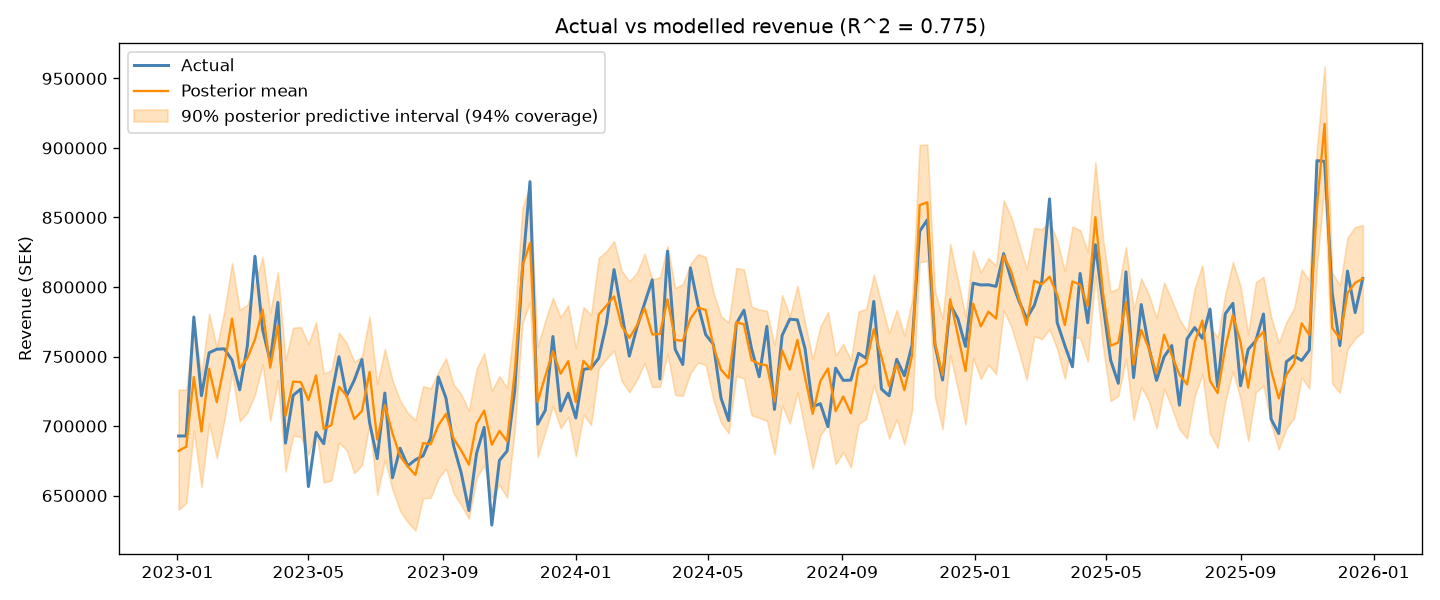
\includegraphics[width=0.95\textwidth]{figures/01_actual_vs_modeled.png}
\caption{Actual weekly revenue (blue) vs posterior-mean prediction (orange) with the 90\% posterior predictive interval (parameter uncertainty plus observation noise). Empirical coverage of the observed revenue is close to the nominal 90\%.}
\end{figure}

\subsection{Parameter recovery}

The posterior 90\% credible interval covers the true value for
\textbf{all 15 channel parameters} (5 channels $\times$ 3 parameters).
Posterior means are typically within one true-value unit but the
intervals are wide because three years of weekly data is a short
identification horizon.

\begin{table}[H]
\centering
\footnotesize
\begin{tabular}{l l r r r r c}
\toprule
\textbf{Channel} & \textbf{Param} & \textbf{True} & \textbf{Mean} & \textbf{5\%} & \textbf{95\%} & \textbf{Covers} \\
\midrule
Search  & $\alpha_{\max}$ & 150\,000 & 168\,155 & 53\,995  & 287\,813 & yes \\
Search  & $\lambda$       & 0.200   & 0.254   & 0.067  & 0.476   & yes \\
Search  & $K$             & 15\,000 & 73\,348  & 11\,895 & 151\,469 & yes \\
Meta    & $\alpha_{\max}$ & 220\,000 & 211\,054 & 121\,219 & 306\,417 & yes \\
Meta    & $\lambda$       & 0.350   & 0.278   & 0.104  & 0.449   & yes \\
Meta    & $K$             & 60\,000 & 59\,604  & 15\,609 & 132\,132 & yes \\
TikTok  & $\alpha_{\max}$ & 150\,000 & 178\,051 & 89\,991 & 275\,297 & yes \\
TikTok  & $\lambda$       & 0.250   & 0.263   & 0.077  & 0.455   & yes \\
TikTok  & $K$             & 40\,000 & 53\,254  & 9\,181  & 134\,990 & yes \\
YouTube & $\alpha_{\max}$ & 65\,000  & 71\,196  & 6\,836  & 171\,504 & yes \\
YouTube & $\lambda$       & 0.450   & 0.336   & 0.081  & 0.620   & yes \\
YouTube & $K$             & 30\,000 & 69\,617  & 2\,553  & 164\,162 & yes \\
Display & $\alpha_{\max}$ & 32\,000 & 85\,757  & 9\,551  & 195\,229 & yes \\
Display & $\lambda$       & 0.200   & 0.296   & 0.067  & 0.580   & yes \\
Display & $K$             & 20\,000 & 76\,123  & 3\,501  & 163\,714 & yes \\
\bottomrule
\end{tabular}
\caption{Posterior recovery of the ground-truth channel parameters. All 15 intervals contain the true value, but interval widths are large because a 156-week panel provides only limited identification.}
\end{table}

\subsection{Revenue decomposition}

\begin{figure}[H]
\centering
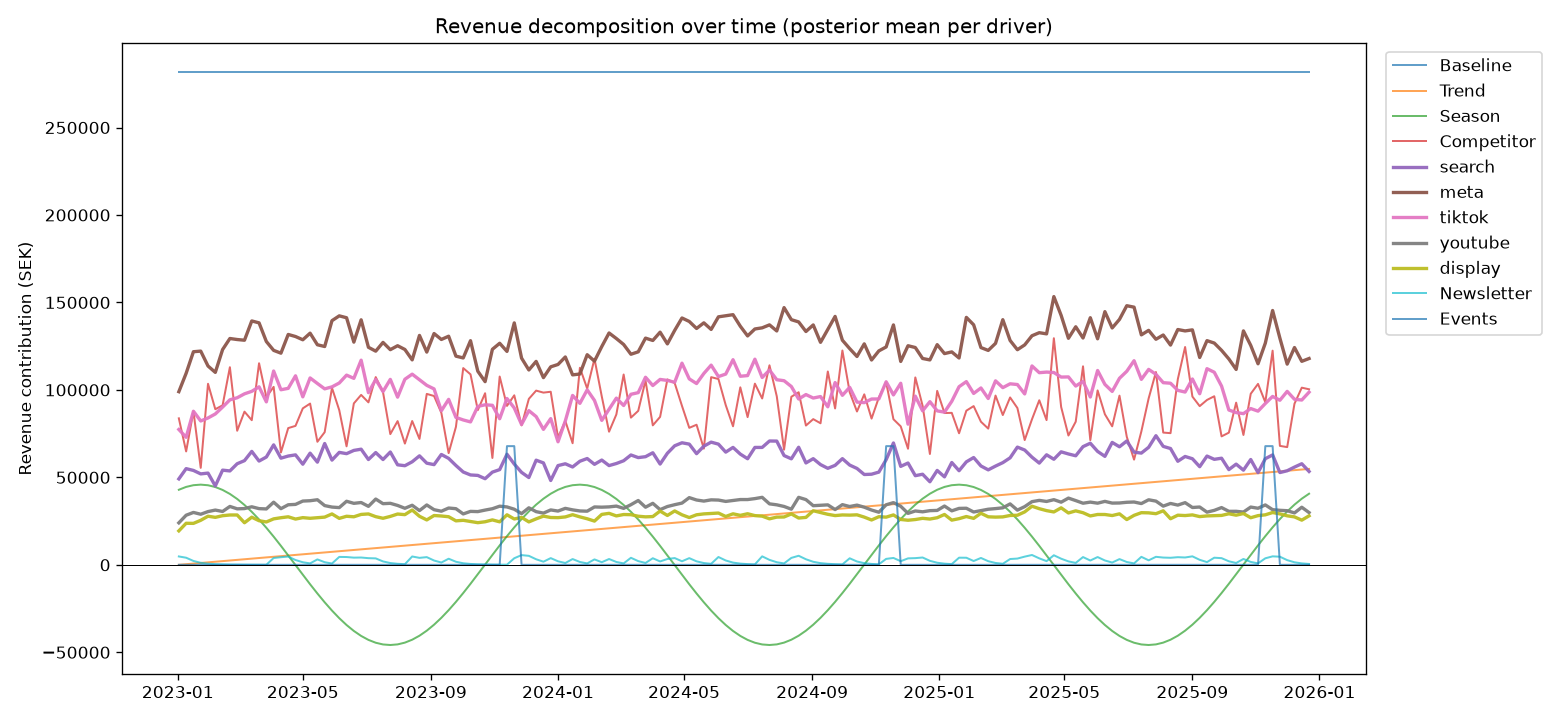
\includegraphics[width=0.95\textwidth]{figures/02_decomposition.png}
\caption{Posterior mean contribution per driver over time. Baseline dominates; channel contributions are the incremental component on top of the always-on level.}
\end{figure}

\begin{table}[H]
\centering
\begin{tabular}{l r r}
\toprule
\textbf{Driver} & \textbf{Contribution (MSEK)} & \textbf{Share} \\
\midrule
Baseline    & 44.0 & 37.5\% \\
Meta        & 19.9 & 17.0\% \\
TikTok      & 15.4 & 13.1\% \\
Competitor  & 14.0 & 11.9\% \\
Search      & 9.4  & 8.0\% \\
YouTube     & 5.2  & 4.4\% \\
Display     & 4.3  & 3.7\% \\
Trend       & 4.3  & 3.7\% \\
Events      & 0.4  & 0.4\% \\
Newsletter  & 0.4  & 0.3\% \\
Season      & 0.0  & 0.0\% \\
\bottomrule
\end{tabular}
\caption{Three-year revenue attribution by driver. Season nets to near-zero because peaks and troughs cancel over an integer number of years.}
\end{table}

\subsection{ROAS per paid channel}

\begin{table}[H]
\centering
\begin{tabular}{l r r r r r}
\toprule
\textbf{Channel} & \textbf{Spend} & \textbf{Contribution} & \textbf{ROAS} & \textbf{5\%} & \textbf{95\%} \\
\midrule
TikTok  & 5\,642\,102 & 15\,381\,013 & 2.73 & 1.00 & 5.52 \\
Search  & 3\,780\,325 & 9\,351\,161  & 2.47 & 0.68 & 5.33 \\
Meta    & 8\,439\,389 & 19\,938\,286 & 2.36 & 1.04 & 4.25 \\
Display & 2\,523\,399 & 4\,328\,926  & 1.72 & 0.14 & 5.60 \\
YouTube & 3\,529\,956 & 5\,203\,248  & 1.47 & 0.09 & 5.30 \\
\bottomrule
\end{tabular}
\caption{ROAS per paid channel with posterior mean and 90\% credible interval. Wide intervals reflect the identification challenge on a 156-week panel with correlated always-on spend.}
\end{table}

\begin{figure}[H]
\centering
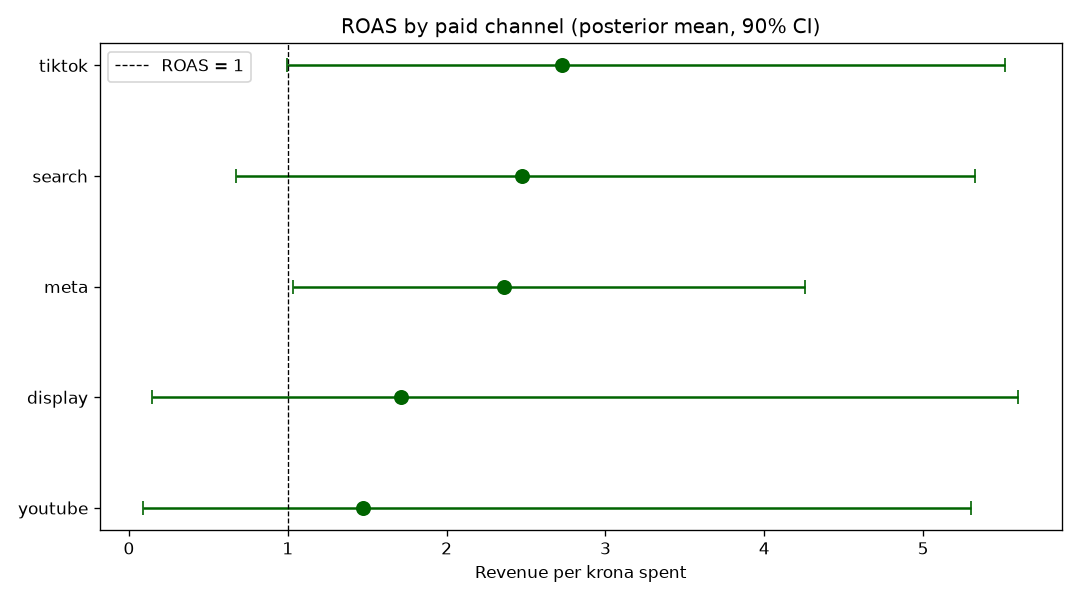
\includegraphics[width=0.85\textwidth]{figures/03_roas.png}
\caption{Posterior mean ROAS per channel with 90\% credible interval. The dashed line marks the break-even point.}
\end{figure}

\section{What the model shows}

The Bayesian MMM in Stan fits weekly revenue well ($R^2 = 0.78$, MAPE
$2.4\%$) and recovers all 15 channel-level ground-truth parameters
inside their 90\% credible intervals. Baseline plus trend explain
about $63\%$ of revenue, which is realistic for retail MMM where
brand and organic demand carry most of the sales.

The main honest weakness is interval width. Posterior means are close
to ground truth on average, but individual parameter intervals span
factors of two or more. This is the fundamental identification
challenge of MMM: three years of weekly data with correlated
always-on channel spend gives the model limited independent variation
to separate channel-level effects from each other and from trend.

Solutions in the rest of the portfolio:
\begin{itemize}
\item Calibration against a geo-lift experiment tightens one channel's
posterior via an informative prior (Project 2).
\item Time-varying coefficients allow channel effectiveness to drift,
which is more realistic than a fixed alpha over three years (Project 3).
\item Bayesian Synthetic Control and BSDID provide the underlying
geo-lift estimator whose posterior feeds back into calibration
(Project 4).
\end{itemize}

\section{Limitations}

\begin{itemize}
\item Synthetic data. The ground-truth generator is stylised. Real
retail data has more complex patterns (promos, stockouts, cross-
category cannibalisation).
\item In-sample fit only. No out-of-time validation.
\item Static coefficients. Channel effectiveness assumed constant over
three years. Project 3 relaxes this.
\item No calibration to lift tests. Project 2 adds this.
\item No cross-channel interaction terms. YouTube-drives-search and
similar effects are not modelled.
\end{itemize}

\section{References}

\begin{itemize}
\item Jin, Wang, Sun, Chan, Koehler (2017).
\emph{Bayesian Methods for Media Mix Modeling with Carryover and Shape
Effects}, Google. Foundational paper for adstock and Hill saturation
in Bayesian MMM.
\item Meta, \emph{Robyn: Semi-Automated MMM}.
\href{https://github.com/facebookexperimental/Robyn}{github.com/facebookexperimental/Robyn}.
\item Google, \emph{Meridian}. \href{https://github.com/google/meridian}{github.com/google/meridian}.
\end{itemize}

\end{document}
